\documentclass{cmn}

\def\cellWidth{9mm}
\def\cellHeight{6mm}
\def\numCells{15}
\def\textWidth{40mm}

\begin{document}
  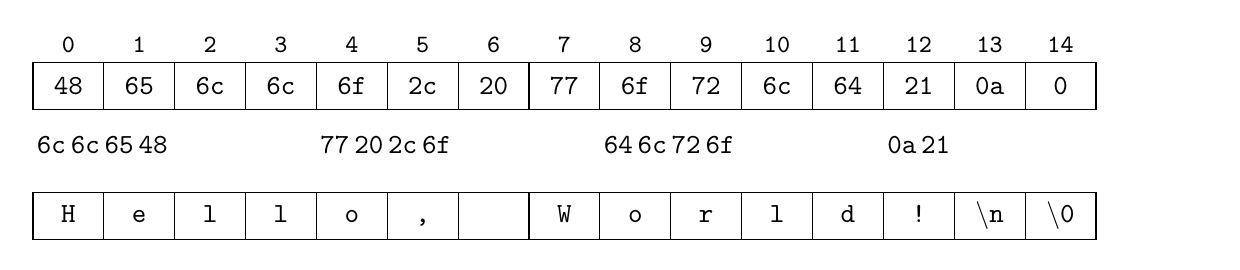
\begin{tikzpicture}
    \pgfmathsetmacro{\lastIndex}{\numCells-1}

    \draw (0,0) -- ++(\numCells*\cellWidth,0) -- ++(0,\cellHeight) -- ++(-\numCells*\cellWidth,0) -- cycle;
    \foreach \i in {1,...,\lastIndex} {
      \draw (\i*\cellWidth,0) -- ++(0,\cellHeight);
    }
    \foreach \i/\t in {1/48,2/65,3/6c,4/6c,5/6f,6/2c,7/20,8/77,9/6f,10/72,11/6c,12/64,13/21,14/0a,15/0} {
      \node at (\i*\cellWidth-0.5*\cellWidth,0.5*\cellHeight) {\texttt{\t}};
    }
    \foreach \i in {0,...,\lastIndex} {
      \node at (\i*\cellWidth+0.5*\cellWidth,1.375*\cellHeight) {\small\texttt{\i}};
    }

    \node[text width=\textWidth,align=left] at (0.5*\textWidth+0.5mm,-0.75*\cellHeight) {\texttt{6c\,6c\,65\,48}};
    \node[text width=\textWidth,align=left] at (4*\cellWidth+0.5*\textWidth+0.5mm,-0.75*\cellHeight) {\texttt{77\,20\,2c\,6f}};
    \node[text width=\textWidth,align=left] at (8*\cellWidth+0.5*\textWidth+0.5mm,-0.75*\cellHeight) {\texttt{64\,6c\,72\,6f}};
    \node[text width=\textWidth,align=left] at (12*\cellWidth+0.5*\textWidth+0.5mm,-0.75*\cellHeight) {\texttt{0a\,21}};

    \draw (0,-2.75*\cellHeight) -- ++(\numCells*\cellWidth,0) -- ++(0,\cellHeight) -- ++(-\numCells*\cellWidth,0) -- cycle;
    \foreach \i in {1,...,\lastIndex} {
      \draw (\i*\cellWidth,-2.75*\cellHeight) -- ++(0,\cellHeight);
    }
    \foreach \i/\t in {0/H,1/e,2/l,3/l,4/o,5/\char44,6/,7/W,8/o,9/r,10/l,11/d,12/!,13/\textbackslash{}n,14/\textbackslash{}0} {
      \node at (\i*\cellWidth+0.5*\cellWidth,-2.25*\cellHeight) {\texttt{\t\vphantom{\strut}}};
    }
  \end{tikzpicture}
\end{document}
